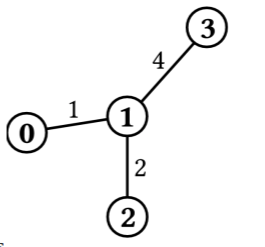
\includegraphics{race1.png}

In the first example, the course can start in city $0$, go to city $1$, and terminate in city $2$. Its length will be exactly $1 + 2 = 3$ km, and it consists of two highways. This is the best possible course; therefore \t{best\_path(N,K,H,L)} must return $2$.

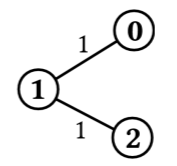
\includegraphics{race2.png}

There is no valid course in the second example. In this case, \texttt{best\_path(N,K,H,L)} must return $-1$.

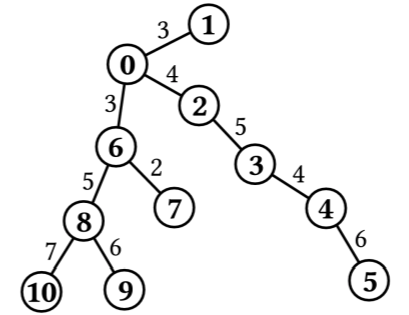
\includegraphics{race3.png}

In the third example, one possible course consists of $3$ highways: from
city $6$ via city $0$ and city $2$ to city $3$. Another course starts in city $10$ and goes via city $8$ to city $6$. Both of these courses have length exactly $12$ km, as required. The second one is optimal, as there is no valid course with a single highway. Hence,
\t{best\_path(N,K,H,L)} must return $2$.